\documentclass{juliacon}
\setcounter{page}{1}

\begin{document}

% **************GENERATED FILE, DO NOT EDIT**************

\title{Explaining Black-Box Models through Counterfactuals}

\author[1]{Patrick Altmeyer}
\author[1]{Arie van Deursen}
\author[1]{Cynthia C. S. Liem}
\affil[1]{Delft University of Technology}

\keywords{Julia, Explainable Artificial Intelligence, Counterfactual Explanations, Algorithmic Recourse}

\hypersetup{
pdftitle = {Explaining Black-Box Models through Counterfactuals},
pdfsubject = {JuliaCon 2022 Proceedings},
pdfauthor = {Patrick Altmeyer, Arie van Deursen, Cynthia C. S. Liem},
pdfkeywords = {Julia, Explainable Artificial Intelligence, Counterfactual Explanations, Algorithmic Recourse},
}



\maketitle

\begin{abstract}

Machine learning models like deep neural networks have become so complex and opaque over recent years that they are generally considered as black boxes. Nonetheless such models often play a key role in modern automated decision-making systems. Counterfactual explanations can help programmers make sense of the systems they build: they explain how inputs into a system need to change for it to produce different decisions. Explanations that involve realistic and actionable changes can be used for the purpose of algorithmic recourse: they offer individuals subject to algorithms a way to turn a negative decision into positive one. In this article we discuss the usefulness of counterfactual explanations for interpretable machine learning and demonstrate its implementation in Julia using the \verb|CounterfactualExplanations| package.

\end{abstract}

\hypertarget{sec-intro}{%
\section{Introduction}\label{sec-intro}}

Advances in technology have typically gone hand in hand with an
outsourcing of labour from humans to machines: the printing press
succeeded human scribes centuries ago, ATMs replaced bank tellers
decades ago and today robots are swarming factory floors. While these
transitions involved a subsitution of manual or repetitive tasks, recent
advances in computing and artificial intelligence (AI) have accelerated
a new type of transformation: from human to data-driven decision-making.
Today, it is more likely than not that your digital loan or employment
application will be handled by an algorithm, at least in the first
instance. This can in theory be beneficial to you: automation typically
leads to increased efficiency and has the potential to remove human bias
and error. In reality though, state-of-the-art algorithms are often
instable (\cite{goodfellow2014explaining}), encode existing biases
(\cite{buolamwini2018gender}) and learn representations that are
surprising or even counter-intuitive form a human perspective
(\textbf{REFERENES?} \cite{}).

This is made more problematic by the fact that many modern machine
learning algorithms tend to be so complex and underspecified in the
data, that they are essentially black boxes. While this is a known
issue, such models are still used to guide decision-making and research
in industry as well as academia. At the time of writing, the largest
artificial neural networks are made up of several hundreds of billion
neurons. In the context of high-stake decision-making systems, black-box
models create undesirable dynamics: the human operators in charge of the
system have to rely on it blindy, while those indviduals subject to it
generally have no way to challenge an outcome. If your digital loan or
employment application gets rejected, for example, that is typically the
end of the story.

\begin{quote}
``You cannot appeal to (algorithms). They do not listen. Nor do they
bend.''

--- Cathy O'Neil in
\href{https://en.wikipedia.org/wiki/Weapons_of_Math_Destruction}{\emph{Weapons
of Math Destruction}}, 2016
\end{quote}

While the inappropriate abuse of such technologies is arguably the
biggest issue, we should also be concerned about missed opportunities.
The lack of trustworthiness in machine learning prevents it from being
adopted in other fields of research, which might actually benefit from
its adoption. Economics and financial markets, for example, are full of
complexities and non-linearities that machine learning algorithms are
well-equipped to model. But financial practitioners and policy makers
are understandably wary of using tools they cannot fully understand
(\cite{oecd2021artificial},\cite{hansen2020virtue}).

In light of all this, a quickly growing body of literature on
explainable artificial intelligence has emerged. Counterfactual
explanations (CE) and algorithmic recourse (AR) fall into this broader
category. Counterfactual explanations can help programmers make sense of
the systems they build: they explain how inputs into a system need to
change for it to produce different decisions. Explanations that involve
realistic and actionable changes can be used for the purpose of
algorithmic recourse (AR): they offer individuals subject to algorithms
a way to turn a negative decision into positive one. Through the
\texttt{CounterfactualExplanations} package we aim to contribute a
scalable and verstile implementation of CE and AR to the Julia
community. The remainder of this article is structured as follows:
Section~\ref{sec-related} presents related work on explainable AI,
Section~\ref{sec-method} provides a brief overview of the methodological
framework, Section~\ref{sec-use} presents the package functionality and
Section~\ref{sec-conclude} concludes.

\hypertarget{sec-related}{%
\section{Related work}\label{sec-related}}

\hypertarget{literature-on-explainable-ai}{%
\subsection{Literature on explainable
AI}\label{literature-on-explainable-ai}}

The field of explainable artificial intelligence (xAI) is still
relatively young and made up of a variety of subdomains, definitions,
concepts and taxonomies. Covering all of these is beyond the scope of
this article, so we will focus only on high-level concepts. The
following literature surveys provide more detail:
\cite{arrieta2020explainable} provide a broad overview of xAI;
\cite{fan2020interpretability} focus on explainability in the context of
deep learning; and finally, \cite{karimi2020survey} offer a detailed
review of the literature on counterfactual explanations and algorithmic
recourse.\footnote{Readers who prefer a text-book approach may also want
  to consider \cite{molnar2020interpretable} and
  \cite{varshney2022trustworthy}}.

The first broad distinction we want to make here is between
\textbf{interpretable} and \textbf{explainable} AI. These terms are
often used interchangeably, but this can lead to confusion. We find the
distinction made in \cite{rudin2019stop} useful: interpretable AI
involves models that are inherently interpretable such as general
additive models (GAM), decision trees and rule-based models; explainable
AI involves models that are not inherently interpretable, but require
additional tools to be explainable to humans. Examples of the latter
include ensembles, support vector machines and deep neural networks.
Some would argue that we best avoid the second category of models
{[}\cite{rudin2019stop}{]} and instead focus solely on interpretable AI.
While we agree that initial efforts should always be geared towards
interpretable models, avoiding black boxes altogether would entail
missed opportunities and anyway is probably not very realistic at this
point. For that reason, we expect the need for explainable AI to persist
in the near future. Explainable AI can further be broadly divided into
\textbf{global} and \textbf{local} explainability: the former is
concerned with explaining the average behaviour of a model, while the
latter involves explanations for individual predictions
\cite{molnar2020interpretable}. Tools for global explainability include
partial dependence plots (PDP), which involves the computation of
marginal effects through Monte Carlo, and global surrogates. A surrogate
model is an interpretable model that is trained to explain the
predictions of a black-box model.

Counterfactual explanations fall into the category of local methods:
they explain how individual predictions change in response to individual
feature perturbations. Among the most popular alternatives to
counterfactual explanations are local surrogate explainers including
local interpretable model-agnostic explanations (LIME) and Shapley
additive explanations (SHAP). They are among the most widely used xAI
tools today, potentially because they are easily understood, relatively
fast and implemented in popular programming languages. Proponents of
surrogate explainers also commonly mention that there is a
straight-forward way to assess their reliability: a surrogate model that
generates predictions in line with those produced by the black-box model
is said to have high fidelity. As intuitive as this notion may be, it
also points to an obvious shoftfall of surrogate explainers: even a
highly fidel surrogate model that produces the same predictions as the
black-box model 99 percent of the time is useless and potentially
misleading for every 1 out 100 individual predictions. In fact, a recent
study has shown that even experienced data scientists tend to put too
much trust in explanations produced by LIME and SHAP
\cite{kaur2020interpreting}. Another recent work has shown that both
LIME and SHAP can be easily fooled: both methods depend on random input
perturbations, a property that be abused by adverse agents to
essentially whitewash strongly biased black-box models
\cite{slack2021fooling}. In a related work the same authors find that
while gradient-based counterfactual explanations can also be
manipulated, there is a straight-forward way to this in practice
\cite{slack2021counterfactual}. In the context of quality assessment, it
is also worth noting that - contrary to surrogate explainers -
counterfactual explanations always achieve full fidelity by
construction: counterfactuals are search with respect to the black-box
classifier, not some approximation of it. That being said,
counterfactual explanations should also be used with care and research
around them is still at its early stages. We shall discuss this in more
detail in Section~\ref{sec-method}.

\hypertarget{existing-software}{%
\subsection{Existing software}\label{existing-software}}

To the best of our knowledge the \texttt{CounterfactualExplanations.jl}
package provides the first implementation of counterfactual explanations
in Julia and therefore represents a novel contribution to the community.
As for other programming languages, we are only aware of one other
unifiying framework: CARLA is Python library that was recently
introduced (\cite{pawelczyk2021carla}). In addition to that, there
exists open-source code for some specific approaches to counterfactual
explanations that have been proposed in recent years. The
approach-specific implementations that we have been able to find are
generally well documented, but exclusively in Python. For example, a
PyTorch implementation of a greedy generator for Bayesian models
proposed in \cite{schut2021generating} can be found
\href{https://github.com/oscarkey/explanations-by-minimizing-uncertainty}{here}.
The popular \href{https://github.com/interpretml}{InterpretML} library
includes an implementation of a diverse counterfactual generator
proposed by \cite{mothilal2020explaining}.

Generally speaking though, software development in the space of xAI has
largely focused on various global methods and surrogate explainers:
implementations of PDP, LIME and SHAP are available for both Python
(e.g.~\href{https://github.com/marcotcr/lime}{\texttt{lime}},
\href{https://github.com/slundberg/shap}{\texttt{shap}}) and R
(e.g.~\href{https://cran.r-project.org/web/packages/lime/index.html}{\texttt{lime}},
\href{https://cran.r-project.org/web/packages/lime/index.html}{\texttt{iml}},
\href{https://modeloriented.github.io/shapper/}{\texttt{shapper}},
\href{https://github.com/bgreenwell/fastshap}{\texttt{fastshap}}). In
the Julia space we have only been able to identify one package that
falls into the broader scope of xAI, namely
\texttt{ShapML.jl}{]}(https://github.com/nredell/ShapML.jl) which
provides an implementation of SHAP. We also should not fail to mention
the comprehensive
\href{https://docs.interpretable.ai/stable/IAIBase/data/}{Interpretable
AI} infrastructure, which focuses exclusively on interpretable models.
Arguably the current availability of tools for explaining black-box
models in Julia is limited, but it appears that the community is
invested in changing that. The team behind \texttt{MLJ.jl}, for example,
is currently recruiting contributors for a project about both
interpretable and explainable AI.\footnote{For details, see the Google
  Summer of Code 2022 project proposal
  \href{https://julialang.org/jsoc/gsoc/MLJ/\#interpretable_machine_learning_in_julia}{here}.}
With our work on counterfactual expanations we hope to contribute to
these efforts. We think that because of its unique transperancy the
Julia language naturally lends itself towards establishing a greater
degree of trust in machine learning and artificial intelligence.

\hypertarget{sec-method}{%
\section{Methodological background}\label{sec-method}}

Counterfactual search happens in the feature space: we are interested in
understanding how we need to change individual attributes in order to
change the model output to a desired value or label
(\cite{molnar2020interpretable}). Typically the underlying methodology
is presented in the context of binary classification:
\(M: \mathcal{X} \mapsto y\) where and \(y\in\{0,1\}\). Let \(t=1\) be
the target class and let \(\overline{x}\) denote the factual feature
vector of some individual outside of the target class, so
\(\overline{y}=M(\overline{x})=0\). We follow this convention here,
though it should be noted that the ideas presented here also carry over
to multi-class problems and regression (\cite{molnar2020interpretable}).

\hypertarget{generic-framework}{%
\subsection{Generic framework}\label{generic-framework}}

Then the counterfactual search objective originally proposed by
\cite{wachter2017counterfactual} is as follows

\begin{equation}\protect\hypertarget{eq-obj}{}{
\min_{\underline{x} \in \mathcal{X}} h(\underline{x}) \ \ \ \mbox{s. t.} \ \ \ M(\underline{x}) = t
}\label{eq-obj}\end{equation}

where \(h(\cdot)\) quantifies how complex or costly it is to go from the
factual \(\overline{x}\) to the counterfactual \(\underline{x}\). To
simplify things we can restate this constrained objective
(Equation~\ref{eq-obj}) as the following unconstrained and
differentiable problem:

\begin{equation}\protect\hypertarget{eq-solution}{}{
\underline{x} = \arg \min_{\underline{x}}  \ell(M(\underline{x}),t) + \lambda h(\underline{x})
}\label{eq-solution}\end{equation}

Here \(\ell\) denotes some loss function targeting the deviation between
the target label and the predicted label and \(\lambda\) governs the
stength of the complexity penalty. Provided we have gradient access for
the black-box model \(M\) the solution to this problem
(Equation~\ref{eq-solution}) can be found through gradient descent. This
generic framework lays the foundation for most state-of-the-art
approaches to counterfactual search and is also used as the baseline
approach - \texttt{GenericGenerator} - in our package. The
hyperparameter \(\lambda\) is typically tuned through grid search.
Conventional choices for \(\ell\) include margin-based losses like
cross-entropy loss and hinge loss. It is worth pointing out that the
loss function is typically computed with respect to logits rather than
predicted probabilities, a convetion that we have chosen to
follow.\footnote{While the rationale for this convention is not entirely
  obvious, implementations of loss functions with respect to logits are
  often numerically more stable. For example, the
  \texttt{logitbinarycrossentropy(ŷ,\ y)} implementation in
  \texttt{Flux.Losses} (used here) is more stable than the
  mathematically equivalent \texttt{binarycrossentropy(ŷ,\ y)}.}

Numerous - and in some cases competing - extensions to this simple
approach have been developed since counterfactual explanations were
first proposed in 2017 (see \cite{verma2020counterfactual} and
\cite{karimi2020survey} for surveys). The various approaches largely
differ in how they define the complexity penalty. In
\cite{wachter2017counterfactual}, for example, \(h(\cdot)\) is defined
in terms of the Manhattan distance between factual and counterfactual
feature values. While this is an intuitive choice, it is too simple to
address many of the desirable properties of effective counterfactual
explanations that have been set out. These desiderata include:
\textbf{closeness} - the average distance between factual and
counterfactual features should be small
(\cite{wachter2017counterfactual}); \textbf{actionability} - the
proposed feature perturbation should actually be actionable
(\cite{ustun2019actionable}, \cite{poyiadzi2020face});
\textbf{plausibility} - the counterfactual explanation should be
plausible to a human (\cite{joshi2019towards}); \textbf{unambiguity} - a
human should have no trouble assigning a label to the counterfactual
(\cite{schut2021generating}); \textbf{sparsity} - the counterfactual
explanation should involve as few individual feature changes as possible
(\cite{schut2021generating}); \textbf{robustness} - the counterfactual
explanation should be robust to domain and model shifts
(\cite{upadhyay2021towards}); \textbf{diversity} - ideally multiple
diverse counterfactual explanations should be provided
(\cite{mothilal2020explaining}); and \textbf{causality} - counterfactual
explanations reflect the structual causal model underlying the data
generating process
(\cite{karimi2020algorithmic},\cite{karimi2021algorithmic}).

\hypertarget{counterfactuals-for-bayesian-models}{%
\subsection{Counterfactuals for Bayesian
models}\label{counterfactuals-for-bayesian-models}}

For what follows it is worth elaborating on the approach proposed in
\cite{schut2021generating}. The authors demonstrate that many of the
abovementioned desiderata can be addressed very easily, if the
classifier \(M\) is Bayesian. In particular, they show that close,
realistic, sparse and unambigous counterfactuals can be generated by
implicitly minimizing the classifier's predictive uncertainty through a
greedy counterfactual search. Formally, they define \(h(\cdot)\) as the
predictive entropy of the classifier, which captures both
\textbf{epistemic} and \textbf{aleatoric} uncertainty: the former is
high on points far away from the training data while the latter is high
in regions of the input space that are inherently noisy. Both are
regions we want to steer clear off in our counterfactual search and
hence predictive entropy is an intuitive choice for a complexity
penalty. The authors further point out that any solution that minimizes
cross-entropy loss (Equation~\ref{eq-solution}) also minimizes
predictive entropy:
\(\arg \min _{\underline{x}} \ell(M(\underline{x}),t) \in \arg \min _{\underline{x}} h(\underline{x})\).
Let \(\mathcal{\widetilde{M}}\) denote the class of binary classifiers
that incorporate predictive uncertainty, then the previous observation
implies that the optimal solution to counterfactual search
(Equation~\ref{eq-solution}) can be restated as follows:

\begin{equation}\protect\hypertarget{eq-solution-bayes}{}{
\underline{x} = \arg \min_{\underline{x}}  \ell(M(\underline{x}),t) \ \ , \ \  \forall M\in\mathcal{\widetilde{M}}
}\label{eq-solution-bayes}\end{equation}

We can drop the complexity penalty altogether and still generate
effective counterfactual explanations. As we will see below, even a fast
and greedy counterfactual search proposed in \cite{schut2021generating}
yields good results in this setting. The approach has been implemented
as \texttt{GreedyGenerator} in our package and should only be used with
classifiers of type \(\mathcal{\widetilde{M}}\). It is worth noting that
the findings in \cite{schut2021generating} are not mutually exclusive of
many of the other methodologies that have been put foward. On the
contrary, we believe that they are complementary: the generic
counterfactual search proposed in \cite{wachter2017counterfactual}, for
example, can be shown to produce more plausible counterfactuals in the
Bayesian setting. Similarly, there is no obvious reason why recent work
on diversity (\cite{mothilal2020explaining}), robustness
(\cite{upadhyay2021towards}) and causality
(\cite{karimi2020algorithmic},\cite{karimi2021algorithmic}) could not be
complemented by the findings in \cite{schut2021generating}. For this
reason we are highlighting \cite{schut2021generating} here and have
prioritized it in the development of
\texttt{CounterfactualExplanations}. While there is no free lunch and
\(M\in\mathcal{\widetilde{M}}\) may seem like a hard constraint, recent
advances in probabilistic machine learning have shown that the
computational cost involved in Bayesian model averaging is lower than we
may have thought (\cite{gal2016dropout},
\cite{lakshminarayanan2016simple}, \cite{daxberger2021laplace},
\cite{murphy2022probabilistic}).

\hypertarget{sec-use}{%
\section{\texorpdfstring{Using
\texttt{CounterfactualExplanations}}{Using CounterfactualExplanations}}\label{sec-use}}

The package is built around two modules that are designed to be as
scalable as possible through multiple dispatch: 1) \texttt{Models} is
concerned with making any arbitrary model compatible with the package;
2) \texttt{Generators} is used to implement arbitrary counterfactual
search algorithms.\footnote{We have made an effort to keep the code base
  a flexible and scalable as possible, but camodelot guarantee at this
  point that really any counterfactual generator can be implemented
  without further adaptation.} The core function of the package
\texttt{generate\_counterfactual} uses an instance of type
\texttt{T\ \textless{}:\ FittedModel} produced by the \texttt{Models}
module (Figure~\ref{fig-models}) and an instance of type
\texttt{T\ \textless{}:\ Generator} produced by the \texttt{Generators}
module (Figure~\ref{fig-generators}). Relating this back the methodology
outlined in Section~\ref{sec-method}, the former instance corresponds to
the model \(M\) while the latter defines the rules for the
counterfactual search (Equation~\ref{eq-solution} and
Equation~\ref{eq-solution-bayes}). In the following we will demonstrate
how to use and extend the package architecture through a few examples.

\begin{figure}

{\centering 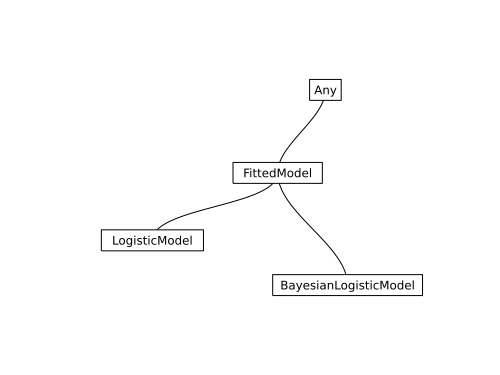
\includegraphics[width=3.33333in,height=2.5in]{www/models.png}

}

\caption{\label{fig-models}Schematic overview of the
\texttt{FittedModel} base type and its descendants.}

\end{figure}

\begin{figure}

{\centering 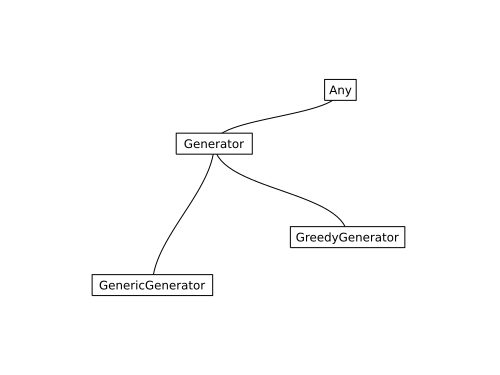
\includegraphics[width=3.33333in,height=2.5in]{www/generators.png}

}

\caption{\label{fig-generators}Schematic overview of the
\texttt{Generator} base type and its descendants.}

\end{figure}

\hypertarget{sec-start}{%
\subsection{Getting started}\label{sec-start}}

The code below provides a complete example demonstrating how the
framework presented in Section~\ref{sec-method} can be implemeted in
Julia using the \texttt{CounterfactualExplantions} package: using a
synthetic data set with linearly separable samples we firstly define our
model and then generate a counterfactual for a randomly selected sample.
Figure~\ref{fig-binary} shows the resulting counterfactual path in the
two-dimensional feature space: features go through iterative
perturbations until the desired confidence level is reached as
illustrated by the contour in the background, which indicates the
classifier's predicted probability that the label is equal to 1.

It may help to go through the relevants parts of the code in some more
detail starting from the part involving the model. For illustrative
purposes the \texttt{Models} module ships with a constructor for a
logistic regression model:
\texttt{LogisticModel(W::Matrix,b::AbstractArray)\ \textless{}:\ FittedModel}.
This constructors does not fit the regression model, but rather takes
its underlying parameters as given. In other words, it is generally
assumed that the user has already estimated a model. Based on the
provided estimates two functions are already implemented that compute
logits and probabilities for the model, respectively. Below we will see
how users can use multiple dispatch to extend these functions for use
with arbitrary models. For now it is enough to note that those methods
define how the model makes its predictions \(M(x)\) and hence they form
an integral part of the counterfactual search.

With the model \(M\) defined in the code below we go on to set up the
counterfactual search as follows: 1) choose a random sample
\texttt{x\_factual}; 2) compute its factual label \texttt{y\_factual} as
predicted by the model (\(M(\overline{x})=0\)); and 3) specify the other
class as our \texttt{target} label (\(t=1\)) along with a desired level
of \texttt{confidence} in the final prediction \(M(\underline{x})=t\).

The last two lines of the code below define the counterfactual generator
and finally run the counterfactual search. The first three fields of the
\texttt{GenericGenerator} are reserved for hyperparameters governing the
strength of the complexity penalty, the step size for gradient descent
and the tolerance for convergence. The fourth field accepts a
\texttt{Symbol} defining the type of loss function \(\ell\) to be used.
Since we are dealing with a binary classification problem logit binary
cross-entropy is an appropriate choice.\footnote{As mentioned earlier,
  the loss function is computed with respect to logits and hence it is
  important to use logit binary cross-entropy loss as opposed to just
  binary cross-entropy.} The fifth and last field can be used to define
mutability constraints for the features.

\begin{lstlisting}[language = Julia]
# Data:
using CounterfactualExplanations, Random
Random.seed!(1234)
N = 100 # number of data points
using CounterfactualExplanations.Data
x, y = toy_data_linear(N) 

# Model:
using CounterfactualExplanations.Models 
w = [1.0 1.0]# true coefficients
b = 0
M = LogisticModel(w, [b])

# Setup:
x_factual = x[rand(1:length(x))]
y_factual = round(probs(M, x_factual)[1])
target = ifelse(y_factual==1.0,0.0,1.0) 
confidence = 0.75 

# Counterfactual search:
generator = GenericGenerator(
    0.1,0.1,1e-5,:logitbinarycrossentropy,nothing)
counterfactual = generate_counterfactual(
    generator, x_factual, M, target, confidence)
\end{lstlisting}

\begin{figure}

{\centering 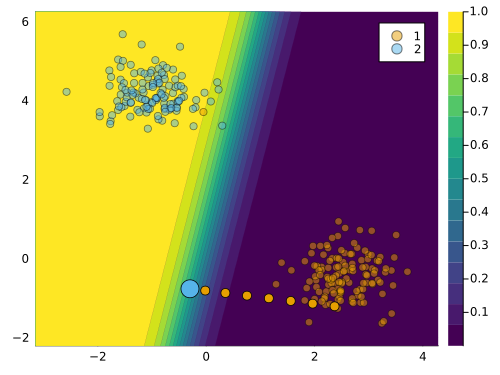
\includegraphics[width=3.33333in,height=2.5in]{www/ce_binary.png}

}

\caption{\label{fig-binary}Counterfactual path using generic
counterfactual generator for conventional binary classifier.}

\end{figure}

In this simple example the generic generator produces an effective
counterfactual: the decision boundary is crossed (i.e.~the
counterfactual explanation is valid) and upon visual inspection the
counterfactual seems plausible (Figure~\ref{fig-binary}). Still, the
example also illustrates that things may well go wrong: since the
underlying model produces high-confidence predictions in regions free of
any data, it is easy to think of scenarios that involve valid but
unrealistic or ambiguous counterfactuals. Consider, for example, the
scenario illustrated in Figure~\ref{fig-binary-wrong}, which involves
the same logisitic classifier albeit massively overfitted. In this case
generic search may yield an unrealistic counterfactual that is well into
the yellow region and yet far away from all other samples (red marker)
or an ambiguous counterfactual near the decision boundary (black
marker).

\begin{figure}

{\centering 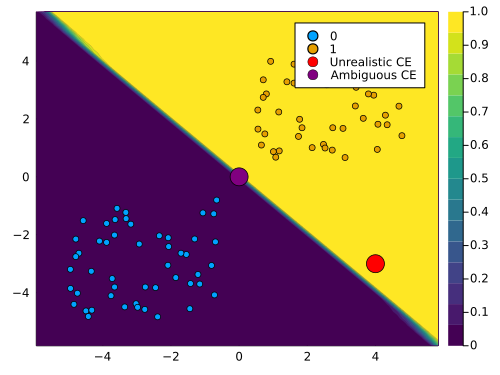
\includegraphics[width=3.33333in,height=2.5in]{www/binary_wrong.png}

}

\caption{\label{fig-binary-wrong}Unrealistic and ambiguous
counterfactuals that may be produced by generic counterfactual search
for an overfitted conventional binary classifier.}

\end{figure}

Among the different approaches that have recently been put forward to
deal with such issues is the greedy generator for Bayesian models
proposed by \cite{schut2021generating}. For reasons discussed in
Section~\ref{sec-method}, we have chosen to prioritize this approach in
the development of \texttt{CounterfactualExplanations}. The code below
shows how this approach can be implemented.
Figure~\ref{fig-binary-laplace} shows the resulting counterfactual path
through the feature space along with the predicted probabilities from
the Bayesian classifier.

Once again it is worth dwelling on the code for a moment. We have used
the same synthetic toy data as before, but this time we use assume that
we have fit a Bayesian logistic regression model through Laplace
approximation. This approximation uses the fact the second-order Taylor
expansion of the logit binary cross-entropy function evaluated at the
maximum-a-posteriori (MAP) estimate amounts to a multivariate Gaussian
distribution (\cite{murphy2022probabilistic}).\footnote{See also this
  \href{https://www.paltmeyer.com/blog/posts/effortsless-bayesian-dl/}{blog
  post} for a gentle introduction and implementation in Julia.} The
\texttt{BayesianLogisticModel\ \textless{}:\ FittedModel} constructor
takes the two moments defining that distribution as its arguments:
firstly, the MAP esitmate, i.e.~the vector of parameters \(\hat\mu\)
including the constant term and, secondly, the corresponding covariance
matrix \(\hat{\Sigma}\). As with logisitic regression above, the package
ships with methods to compute predictions from instances of type
\texttt{BayesianLogisticModel}.\footnote{Predictions are computed using
  a probit approximation.} Contrary to the simple logisitic regression
model above, predictions from the Bayesian logistic model incorporate
uncertainty and hence predicted probabilities fan out in regions free of
any training data (Figure~\ref{fig-binary-laplace}).

For the counterfactual search we use a greedy approach following
\cite{schut2021generating}. The approach is greedy in the sense that in
each iteration it selects the most salient feature with respect to our
objective (Equation~\ref{eq-solution-bayes}) and perturbs it by some
predetermined step size \(\delta\). Since the gradient
\(\nabla_{\underline{x}}\ell(M(\underline{x},t))\) in this case is
proportional to the MAP estimate \(\hat\mu\), the same feature is chosen
until a predefined maximum number of perturbations \(n\) has been
exhausted. Those two hyperparameters, \(\delta\) and \(n\), are defined
in the first two fields of
\texttt{GreedyGenerator\ \textless{}:\ Generator} in the code below. The
third and fourth field are reserved for the loss function and mutability
constraints. Since we are making use of multiple dispatch, the final
command that actually runs the counterfactual search is the same as
before.

\begin{lstlisting}[language = Julia]
# Model:
using LinearAlgebra
I = UniformScaling(1)
cov = Symmetric(reshape(randn(9),3,3).*0.01 + I) 
w = [1 1]
coeffs = hcat(b, w)
M = BayesianLogisticModel(coeffs, cov)

# Counterfactual search:
generator = GreedyGenerator(
    0.25,20,:logitbinarycrossentropy,nothing)
counterfactual = generate_counterfactual(
    generator, x_factual, M, target, confidence)
\end{lstlisting}

The counterfactual in Figure~\ref{fig-binary-laplace} is not only valid,
but also realistic and unambiguous. In this case it is more difficult to
imagine adverse scenarios like in Figure~\ref{fig-binary-wrong}.
Evidently it is easier to avoid pitfalls when generating counterfactual
explanations for models that incorporate predictive uncertainty.

\begin{figure}

{\centering 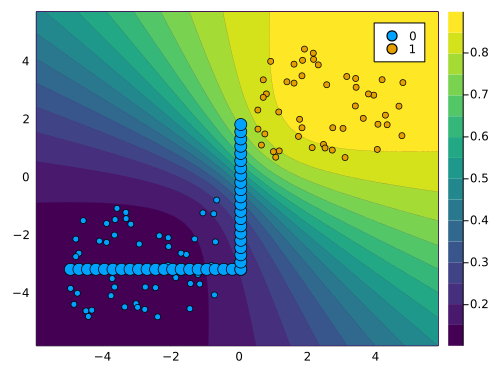
\includegraphics[width=3.33333in,height=2.5in]{www/ce_binary_laplace.png}

}

\caption{\label{fig-binary-laplace}Counterfactual path using greedy
counterfactual generator for Bayesian binary classifier.}

\end{figure}

\hypertarget{sec-custom}{%
\subsection{Custom models}\label{sec-custom}}

One of our priorities has been to make
\texttt{CounterfactualExplanations} scalable and versatile. In the long
term we aim to add support for more default models and counterfactual
generators. In the short term it is designed to allow users to integrate
models and generators themselves. Ideally, these community efforts will
facilitate our long-term goals. Only two steps are necessary to make any
supervised-learning model compatible with our package\footnote{In order
  for the model to be compatible with the gradient-based default
  generators presented in Section~\ref{sec-start} gradient access is
  also necessary, but any model can also be complemented with a custom
  generator.}:

To demonstrate how this can be done in practice we will now consider
another synthetic example. Once again samples are two-dimensional for
illustration purposes, but this time they are grouped into four
different classes and not linearly separable. To predict class labels
based on features we use a simple deep-learning model trained in
\href{https://fluxml.ai/}{Flux.jl} (\cite{innes2018flux}). The code
below shows the simple model architecture. Note how outputs from the
final layer are note passed through a softmax activation function, since
counterfactual loss is evaluated with respect to logits as we discussed
earlier. The model is trained with dropout for ten training epochs.

\begin{lstlisting}[language = Julia]
n_hidden = 32
output_dim = length(unique(y))
input_dim = 2
model = Chain(
    Dense(input_dim, n_hidden, activation),
    Dropout(0.1),
    Dense(n_hidden, output_dim)
)  
\end{lstlisting}

The code below implements the two steps that are necessary to make the
trained neural network compatible with the package: subtyping and
multiple dispatch. Computing logits amounts to just calling the Flux.jl
model on inputs. Predicted probabilities for labels can than be computed
through softmax.

\begin{lstlisting}[language = Julia]
# Step 1)
struct NeuralNetwork <: Models.FittedModel
    model::Any
end

# Step 2)
# import functions in order to extend
import CounterfactualExplanations.Models: logits
import CounterfactualExplanations.Models: probs 
logits(M::NeuralNetwork, X::AbstractArray) = M.model(X)
probs(M::NeuralNetwork, X::AbstractArray) = softmax(logits(M, X))
M = NeuralNetwork(model)
\end{lstlisting}

Finally, the code below draws a random sample and generates a
counterfactual in a different target class through generic search. The
code very much resembles the earlier examples, with the only notable
difference that for the counterfactual loss function we are now using
the multi-class logit cross-entropy loss. The resulting counterfactual
path is shown in Figure~\ref{fig-multi}. In this case the contour shows
the predicted probability that the input is in the target class
(\(t=4\)). Generic search yields a valid, realistic and unambiguous
counterfactual.

\begin{lstlisting}[language = Julia]
# Randomly selected factual:
using Random
Random.seed!(42)
x_factual = x[rand(1:length(x))]
y_factual = Flux.onecold(
    probs(M, x_factual),unique(y))
target = rand(unique(y)[1:end .!= y_factual]) 
confidence = 0.75

# Counterfactual search:
generator = GenericGenerator(
    0.1,0.1,1e-5,:logitcrossentropy,nothing)
counterfactual = generate_counterfactual(
    generator, x_factual, M, target, confidence)
\end{lstlisting}

\begin{figure}

{\centering 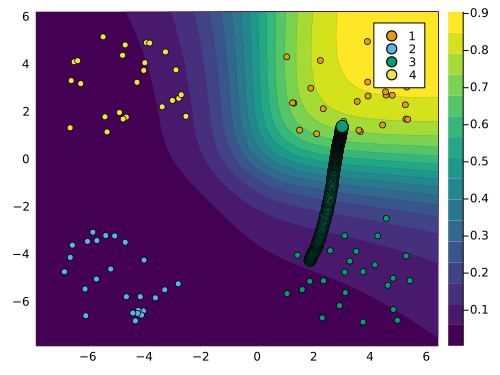
\includegraphics[width=3.33333in,height=2.5in]{www/ce_multi.png}

}

\caption{\label{fig-multi}Counterfactual path using generic
counterfactual generator for multi-class classifier.}

\end{figure}

As before we will also look at the Bayesian setting. One way to
incorporate predictive uncertainty in deep learning is through a deep
ensemble (\cite{lakshminarayanan2016simple}). Using we can recover a
Bayesian representation of our neural network in a post-hoc fashion .
Alternatively, we could have Monte Carlo dropout
(\cite{gal2016dropout}), variational inference or Laplace approximation
(LA) much in the same way as above (\cite{daxberger2021laplace}). Using
the greedy generator for the deep ensemble yields the counterfactual
path in Figure~\ref{fig-multi-ensemble}. The code that produces these
results follows below.

\begin{lstlisting}
# Deep ensemble:
using Flux: stack
# Step 1)
struct FittedEnsemble <: Models.FittedModel
    ensemble::AbstractArray
end
# Step 2)
using Statistics
logits(M::FittedEnsemble, X::AbstractArray) = mean(
    stack([m(X) for m in M.ensemble],3), 
    dims=3)
probs(M::FittedEnsemble, X::AbstractArray) = mean(
    stack([softmax(m(X)) for m in M.ensemble],3),
    dims=3)
M_ensemble = FittedEnsemble(ensemble)
\end{lstlisting}

Contrary to the example involving binary classification above, it is
less clear that counterfactuals for the Bayesian classifier are more
effective in this case. Predictions from this simple deep ensemble look
very similar to those produced by the MLP: the model fails to only
produce high-confidence predictions in regions that are abundant with
training samples. This illustrates that the quality of counterfactual
explanations may ultimately depend to some degree on the quality of the
classifier. Put differently, if the quality of the classifier is poor,
we may expect this to come through in the counterfactual explanation.

\begin{figure}

{\centering 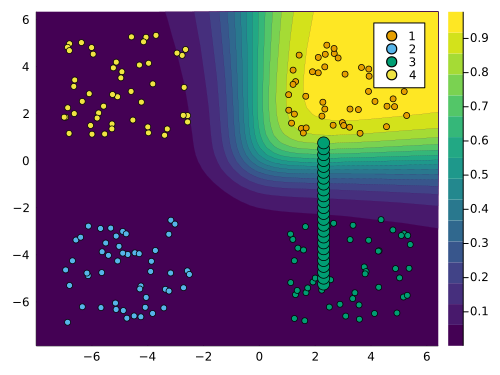
\includegraphics[width=3.33333in,height=2.5in]{www/ce_multi_ensemble.png}

}

\caption{\label{fig-multi-ensemble}Counterfactual path using generic
counterfactual generator for multi-class classifier with Laplace
approximation.}

\end{figure}

\hypertarget{laguage-interoperability}{%
\subsection{Laguage interoperability}\label{laguage-interoperability}}

The Julia language offers unique support for programming language
interoperability. For example, calling R or Python is made remarkably
easy through \texttt{RCall.jl} and \texttt{PyCall.jl}, respectively.
This functionality can be leveraged to use
\texttt{CounterfactualExplanations.jl} to generate explanations for
models that were developed in other programming languages. While at the
time of writing we have not yet implemented out-of-the-box support for
foreign programming languages, the following example demonstrates how
versatile our package is.

\hypertarget{explaining-a-model-trained-in-r}{%
\subsubsection{\texorpdfstring{Explaining a model trained in
\texttt{R}}{Explaining a model trained in R}}\label{explaining-a-model-trained-in-r}}

We have trained a simple MLP using the R library \texttt{torch} for
binary classification task involving a synthetic data set. Inside the R
working environment the fitted \texttt{torch} model is stored as an
object called \texttt{model}. That R object can be accessed from Julia
using \texttt{RCall.jl} by simply calling \texttt{R"model"}. As in
Section~\ref{sec-custom} and Section~\ref{sec-emp} the first thing
necessary to make that model compatible with our package is to declare
it as a subtype of \texttt{Model.FittedModel}. As always we also need to
extend the \texttt{logits} and \texttt{probs} functions to make the
model compatible with \texttt{CounterfactualExplanations.jl}. The code
below shows how this can be done. Logits are returned by the
\texttt{torch} model and copied from R into the Julia environment.
Probabilities are then computed in Julia by passing the logits through
the sigmoid function.

\begin{lstlisting}
# Step 1)
struct TorchNetwork <: Models.FittedModel
    nn::Any
end

# Step 2)
function logits(M::TorchNetwork, X::AbstractArray)
    nn = M.nn
    y = rcopy(R"as_array($nn(torch_tensor(t($X))))")
    y = isa(y, AbstractArray) ? y : [y]
    return y
end
function probs(M::TorchNetwork, X::AbstractArray)
    Flux.sigmoid.(logits(M, X))
end
M = TorchNetwork(R"model")
\end{lstlisting}

Next we need to do a tiny bit of work on the \texttt{Generator} side.
The default methods underlying the counterfactual generators are desiged
to work with models that have gradient access through
\texttt{Zygote.jl}, one of Julia's main autodifferentiation packages. Of
course, \texttt{Zygote.jl} cannot access the gradients of our
\texttt{torch} model, so we need to adapt the code slightly.
Fortunately, it turns out that all we need to do is extend the function
that computes the gradient with respect to the loss function for the
generic counterfactual search. In particular, we will extend the
function by a method that is specific to the \texttt{TorchNetwork} type
we defined above. The code below implements this: our new method calls R
in order to use \texttt{torch}'s autodifferentiation functionality for
computing the gradient.

\begin{lstlisting}
import CounterfactualExplanations.Generators: grad_loss
using LinearAlgebra

# Countefactual loss:
function grad_loss(generator::GenericGenerator, x, M::TorchNetwork, t) 
  nn = M.nn
  R"""
  x <- torch_tensor($x, requires_grad=TRUE)
  output <- $nn(x)
  loss_fun <- nnf_binary_cross_entropy_with_logits
  obj_loss <- loss_fun(output,$t)
  obj_loss$backward()
  """
  grad = rcopy(R"as_array(x$grad)")
  return grad
end
\end{lstlisting}

From here on onwards the \texttt{CounterfactualExplanations.jl}
functionality can be used as always. Figure~\ref{fig-torch} shows the
counterfactual path for a randomly chosen sample with respect to the MLP
trained in R.

\begin{figure}

{\centering 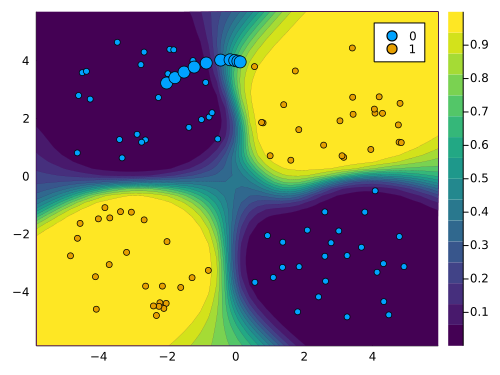
\includegraphics[width=3.33333in,height=2.5in]{www/ce_torch.png}

}

\caption{\label{fig-torch}Counterfactual path using generic
counterfactual generator for a model trained in R.}

\end{figure}

\hypertarget{explaining-a-model-trained-in-python}{%
\subsubsection{Explaining a model trained in
Python}\label{explaining-a-model-trained-in-python}}

\textbf{TO ADD, MAYBE}

\hypertarget{sec-emp}{%
\subsection{Empirical example}\label{sec-emp}}

Now that we have explained the basic functionality of
\texttt{CounterfactualExplanations} through a few illustrative toy
examples, it is time to consider some real data. The MNIST dataset
contains 60,000 training samples of handwritten digits in the form of
28x28 pixel grey-scale images (\cite{lecun1998mnist}). Each image is
associated with a label indicating the digit (0-9) that the image
represents. The data makes for an interesting case-study of
counterfactual explanations, because humans have a good idea of what
realistic counterfactuals of digits look like. For example, if you were
asked to pick up an eraser and turn the digit in
Figure~\ref{fig-mnist-orig} into a four (4) you would know exactly what
to do: just erase the top part. In \cite{schut2021generating} leverage
this idea to illustrate to the reader that their methodolgy produces
effective counterfactuals. In what follows we replicate some of their
findings. You as the reader are therefore the perfect judge to evaluate
the quality of the counterfactual explanations presented here.

On the model side we will use two pre-trained classifiers\footnote{The
  pre-trained models were stored as package artifacts and loaded through
  helper functions.}: firstly, a simple multi-layer perceptron (MLP)
and, secondly, a deep ensemble composed of five such MLPs following
\cite{schut2021generating}. Deep ensembles are approximate Bayesian
model averages that have been shown to yield high-quality esimtates of
predictve uncertainty for neural networks (\cite{wilson2019case.pdf},
\cite{lakshminarayanan2016simple})). In the previous section we already
created the necessary subtype and methods to make the multi-output MLP
compatible with our package. The code below implements the two necessary
steps for the deep ensemble.

\begin{lstlisting}
using Flux: stack
# Step 1)
struct FittedEnsemble <: Models.FittedModel
    ensemble::AbstractArray
end
# Step 2)
using Statistics
logits(M::FittedEnsemble, X::AbstractArray) = mean(
    stack([m(X) for m in M.ensemble],3), 
    dims=3)
probs(M::FittedEnsemble, X::AbstractArray) = mean(
    stack([softmax(m(X)) for m in M.ensemble],3),
    dims=3)
M_ensemble = FittedEnsemble(ensemble)
\end{lstlisting}

\begin{figure}

{\centering 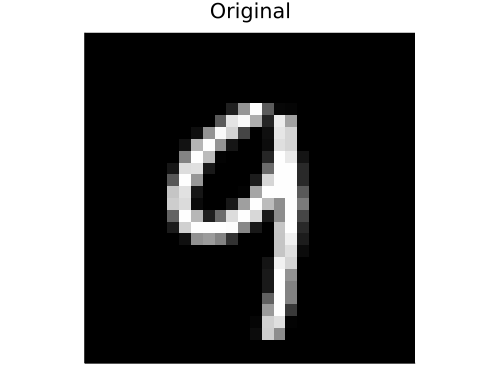
\includegraphics[width=1.66667in,height=1.25in]{www/mnist_original.png}

}

\caption{\label{fig-mnist-orig}A handwritten nine (9) randomly drawn
from the MNIST dataset.}

\end{figure}

For the counterfactual search we will use four different combinations of
classifiers and generators: firstly, the generic approach for the MLP;
secondly, the greedy approach for the MLP; thirdly, the generic approach
for the deep ensemble; and finally, the greedy approach for the deep
ensemble.

We begin by turning the nine in Figure~\ref{fig-mnist-orig} into a four.
Figure~\ref{fig-mnist-9to4} shows the resulting counterfactuals. In
every case the desired label switch is in fact achieved, but arguably
from a human perspective only the counterfactuals for the deep ensemble
look like a four. The generic generator produces mild perturbations in
regions that seem irrelevant from a human perspective, but nonetheless
yields a coutnerfactual that can pass as a four. The greedy approach
(\cite{wacther2021generating}) clearly targets pixels at the top of the
handwritten nine and yields the best result overall. For the
non-bayesian MLP, both the generic and the greedy approach generate
counterfactuals that look much like adversarial examples: they perturb
pixels in seemingly random regions on the image.
Figure~\ref{fig-mnist-3to8} shows another example. This time the goal is
to turn a randomly chosen three (3) into an eight (8). Onve again the
outcomes for the deep ensemble look more realistic, but overall the
generated counterfactuals look less effective than those in
Figure~\ref{fig-mnist-9to4}. The results could likely be improved by
using adversarial training for the classifiers as recommended in
\cite{wachter2021generating}

\begin{figure}

{\centering 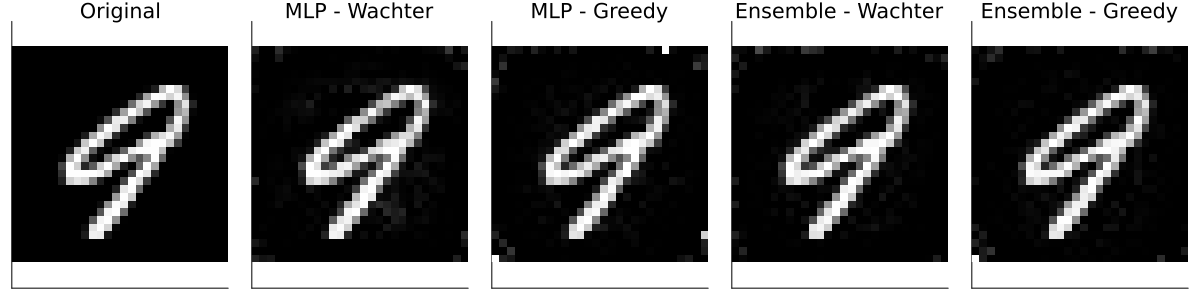
\includegraphics[width=3.33333in,height=0.83333in]{www/mnist_9_to_4.png}

}

\caption{\label{fig-mnist-9to4}Counterfactual explanations for MNIST:
turning a nine (9) into a four (4)}

\end{figure}

Overall, the examples in this section demonstrate two points that we
have already made earlier: firstly, the findings in
\cite{wachter2021generating} can indeed complement other existing
approaches to counterfactual generation; and secondly, the quality of
the classifier is clearly reflected in the quality of the counterfactual
explanations. In other words, we cannot generate effective
counterfactual explanations for a poorly trained model. That is actually
desirable: if a model bases its predictions on representations that are
not intuitive to a human, we would like that to be evident from the
counterfactual explanation. From that perspective, counterfactual
explanations can help us to not only understand a black-box model, but
potentially also guide us in improving it.

\begin{figure}

{\centering 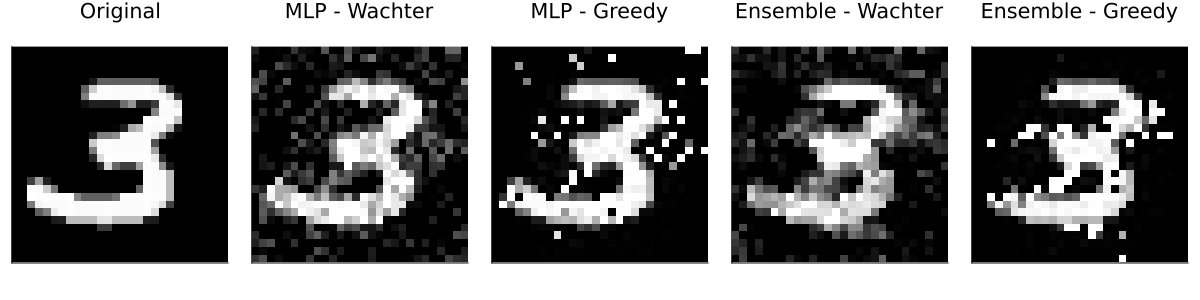
\includegraphics[width=3.33333in,height=0.83333in]{www/mnist_3_to_8.png}

}

\caption{\label{fig-mnist-3to8}Counterfactual explanations for MNIST:
turning a three (3) into an eight (8)}

\end{figure}

\hypertarget{sec-conclude}{%
\section{Concluding remarks}\label{sec-conclude}}

In this article has introduced \texttt{CounterfactualExplanation.jl}: a
package for generating counterfactual explanations and algorithmic
recourse in Julia. We have argued that these are particularly promising
tools for explaining black-box models. Through various examples we have
shown how to use and extend the package. It is designed to allow users
to generate counterfactual explanations for their own custom models and
using their own custom generators. Thanks to Julia's support for
language interoperability, \texttt{CounterfactualExplanation.jl} can
even explain models that were developed and trained in other programming
languages as we have demonstrated through an example of a deep neural
network trained in R \texttt{torch}. We believe that this package in its
current form offers a valuable contribution to ongoing efforts towards
explainable artificial intelligence by the broader Julia community. That
being said, there is significant scope for further development. At the
time of writing the package supports only a few default models and
generators natively. Through future work on our side and contributions
through the community we plan to expand its functionality further.

% **************GENERATED FILE, DO NOT EDIT**************

\bibliographystyle{juliacon}
\bibliography{ref.bib}


\end{document}
